\part{Data analysis}
\label{part:data_analysis}

%------------------------------------

\section{About this part}
\label{section:DA_about_part}
Before rigorously testing different models available, it's important to take a look at the data that is supplied.
The supplied data consists of two main groups of images, labelled training images and unlabeled test images.
As per the requirements of the Kaggle competition, the test images should only be used for evaluating the model.
Thus the test images \textit{can not} be used for creating the model in any shape or form.
This means that only the labelled training images can be used to create and validate the model in development.
To avoid altering the model to perform well on the supplied test data and not in general, only the training data will be analysed.
All code used for this part is available under the developed code folder on GitHub, in the Jupyter Notebook \texttt{data\_analysis.ipynb}.
This part will only analyze the data and make suggestions for possible preprocessing, it won't manipulate the data just yet.
This notebooks allows for changing parameters easily, which is crucial since this analysis has to be done for multiple descriptors and settings.

%------------------------------------

\section{Data distribution}
\label{section:DA_data_distribution}
The provided labeled training data consists of 12 different classes.
There is a total of 4042 labelled training images supplied, the distribution of which is shown in figure \ref{fig:1-data_analysis-labeled_data_distribution}.
As visible in this figure, the distribution between classes is not balanced.
This has to be taken into account when fitting a model since some models will show unwanted behaviour when fitted with unbalanced data.
Luckily many solutions exist to minify the impact of this unbalance.
This unbalance has to be kept in mind when using a split of the training set as a validation set as well.
This is because such split might lead to a test set where some classes have considerably fewer instances in the test set and thus the performance on those classes has less impact on the total score, which may be unwanted.

\begin{figure}[H]
    \centering
    \fbox{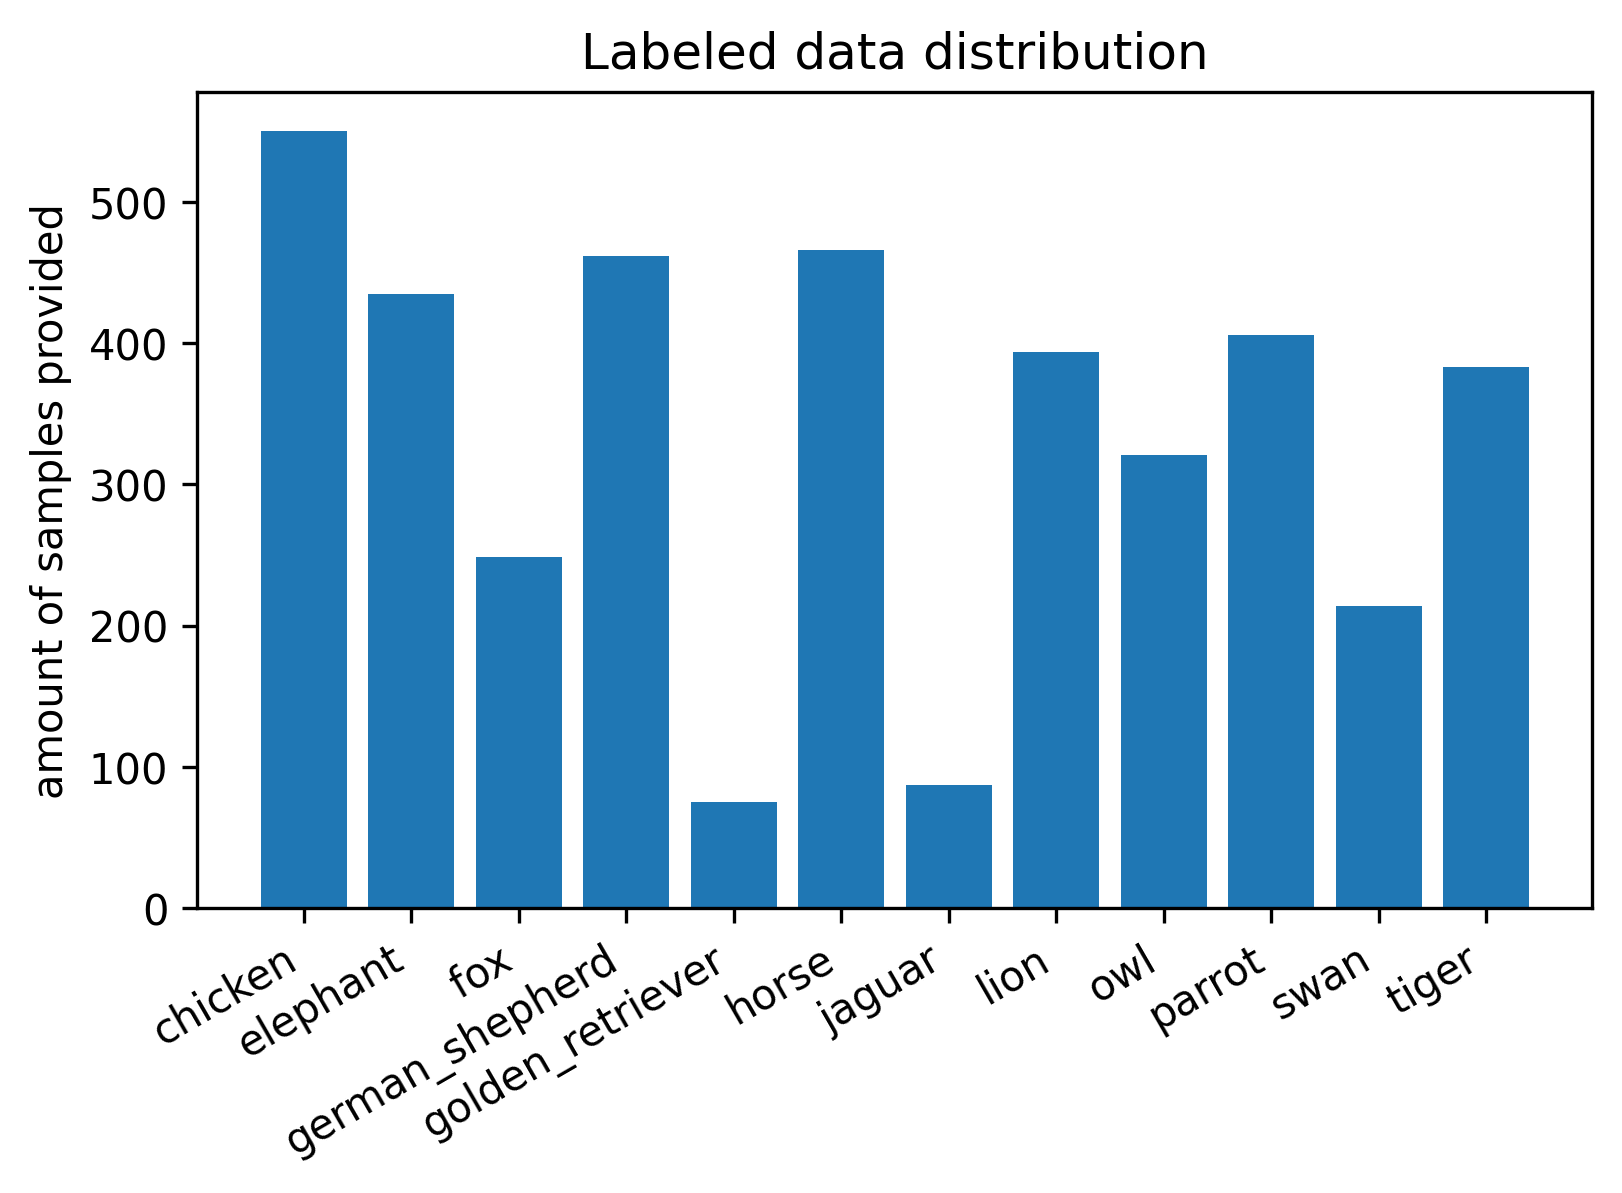
\includegraphics[width=0.65\linewidth]{images/1/1-data_analysis-labeled_data_distribution.png}}
    \captionsetup{width=0.6\linewidth}
    \captionsetup{justification=centering}
    \caption{Data distribution training data.}
    \label{fig:1-data_analysis-labeled_data_distribution}
\end{figure}

%------------------------------------

\section{Deeper look at the training data}
\label{section:DA_deeper_look_data}

Whilst noting that the available data isn't balanced over all the classes is very important, there are also different aspects of the data that need analysing. 
An overview of the supplied training data is given in figure \ref{fig:1-data_analysis-labeled_data_overview.png}, available in the figures list at the end of this report.
This figure shows the first five images of each class.
From this, it becomes apparent that multiple factors of the data aren't \emph{optimal}.
This knowledge is important since it can aid in better prepossessing and in finding a better model in general.
The most noteworthy findings are listed here:
\begin{itemize}
    \item Images vary in shapes, some are taken in portrait, others in landscape.
    \item Images vary in size, some are high resolution whilst others are relatively low resolution.
    \item The framing of the subject(s) varies a lot. Sometimes the labelled animal is completely visible and centred in the frame. In some images there are multiple animals spread across the image, others show a close-up of the animal.
    \item Some images have a detailed background that makes up for a lot of the image, in others the background is blurry and its impact is presumably less.
    \item Some images have very vibrant colours in broad daylight, others are black and white in dimly lit environments.
\end{itemize}

This diversity in the provided training set is expected since it has been scraped from the web.
This also means that \emph{noise} can be expected, another important factor to keep in mind when choosing and optimizing models.
Many of the listed things can be minified by doing some clever prepossessing of the images.


%------------------------------------

\section{Feature extraction}
\label{section:DA_feature_extraction}

Some feature extraction has already been provided.
In short, images are converted from there typical RGB representation to a numerical representation of interesting points, which can be used as input for our model.
How this is done and could be optimized is briefly discussed here.

Instead of using the whole image as data, only a select few of \textit{interesting points} of the image are taken into consideration.
These interesting points of an image are found by using the \emph{Shi-Tomasi corner detector}.
As the name suggest, these interesting points are \textit{strong corners on an image}.
The following important parameters for the \texttt{features.extractShiTomasiCorners} function call are:
\begin{itemize}
    \item Maximum number of interesting points = 500
    \item Minimum Euclidean distance between interesting points = 20
\end{itemize}

\clearpage
Shown in figure \ref{fig:1-poi} is an example output of interesting points found by the Shi-Tomasi corner detector.
It's clear that it's performance varies a lot, but finding interesting points isn't an easy task and thus the results are better then they might seem on first sight.
This method might benefit from fine-tuning and earlier preprocessing of the data.

\begin{figure*}[ht]
    \centering
    \begin{subfigure}{.35\textwidth}
        \centering
        \fbox{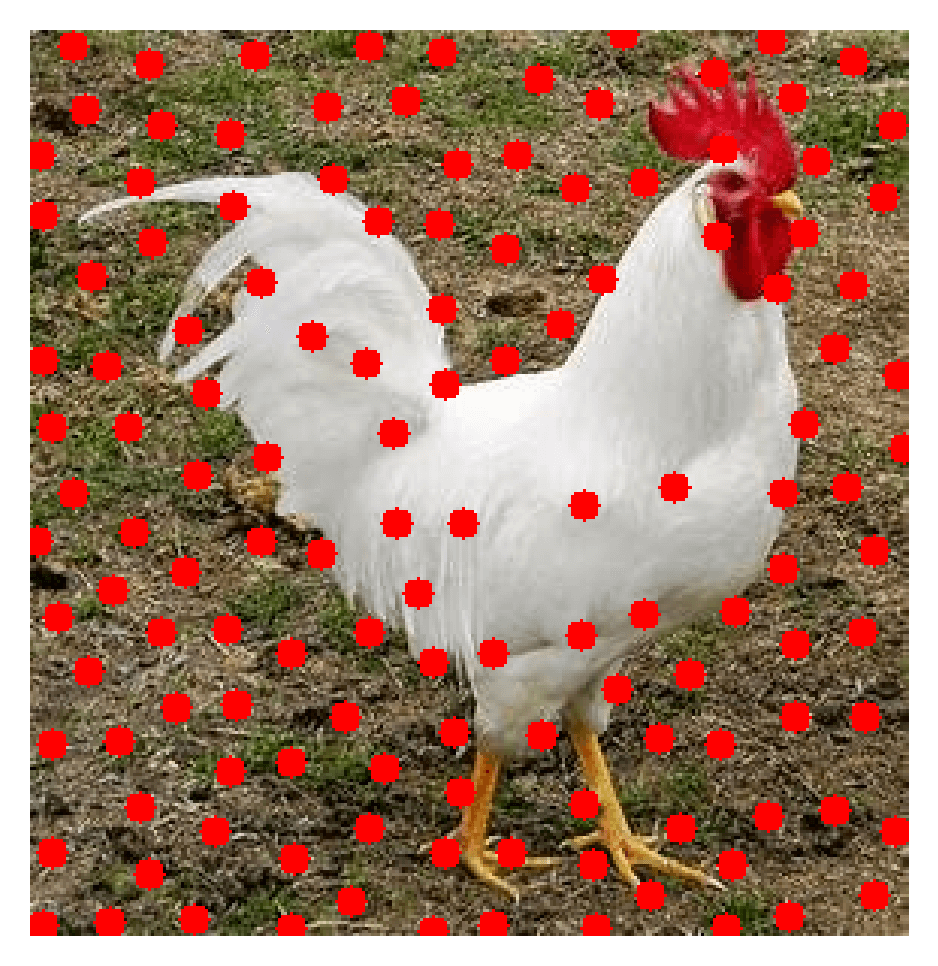
\includegraphics[width=\textwidth]{images/1/1-data_analysis-POI_chicken.png}}
        \captionsetup{width=0.9\linewidth}
        \captionsetup{justification=centering}
        \caption{First chicken from train data.}
    \end{subfigure}
    \hspace{1cm}
    \begin{subfigure}{.52\textwidth}
        \centering
        \fbox{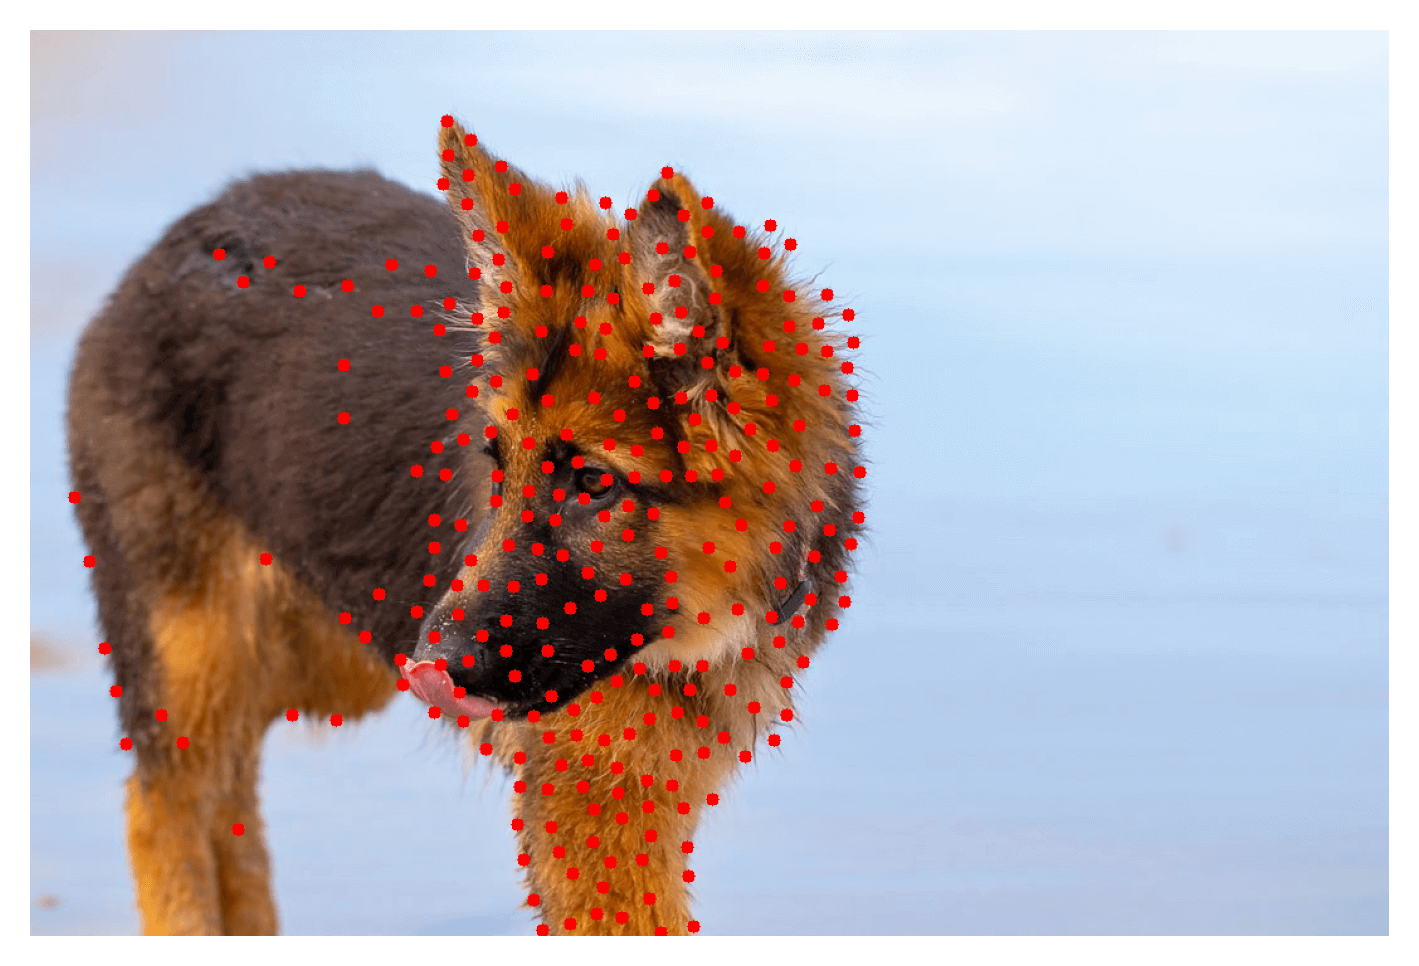
\includegraphics[width=\textwidth]{images/1/1-data_analysis-POI_german_shepherd.png}}
        \captionsetup{width=0.9\linewidth}
        \captionsetup{justification=centering}
        \caption{First German shepherd from train data}
    \end{subfigure}
    \captionsetup{width=0.8\linewidth}
    \captionsetup{justification=centering}
    \caption{Points of interest found by the Shi-Tomasi corner detector.}
    \label{fig:1-poi}
\end{figure*}


%------------------------------------

\section{The numerical representation}
\label{section:DA_numerical_representation}

Finding interesting points is only half of the work.
These interesting points now need to be represented by numerical values that have actual meaning.
Remember from section \ref{section:DA_deeper_look_data} that the provided images differ a lot.
Thus the numerical representation, generated by a descriptor, has to be so that it minifies the impact of different lighting, scaling...
afterwards, these values can be clustered together.
Clustering is done by the \texttt{createCodebook} function which uses Mini-Batch K-Means clustering from the SciKit Learn library.
Opting for a different clustering algorithm and/or fine-tuning its (hyper)parameters might result in better performance of the chosen model.

An overview showing histograms for each word (cluster) and a corresponding correlation matrix is shown in figure \ref{fig:1-cm}.
From the histogram, it is visible that the values are normalized as was discussed.
This would have to be checked for all descriptors used and perhaps some outliers would need to be removed.
The correlation between these clusters doesn't seem too dramatic when opting for 30 clusters.
A low correlation between clusters is mostly positive for model building since it means each cluster represent a distinct concept.
This is again something that would have to be checked for different parameters.

\begin{figure*}[ht]
    \centering
    \begin{subfigure}{.45\textwidth}
        \centering
        \fbox{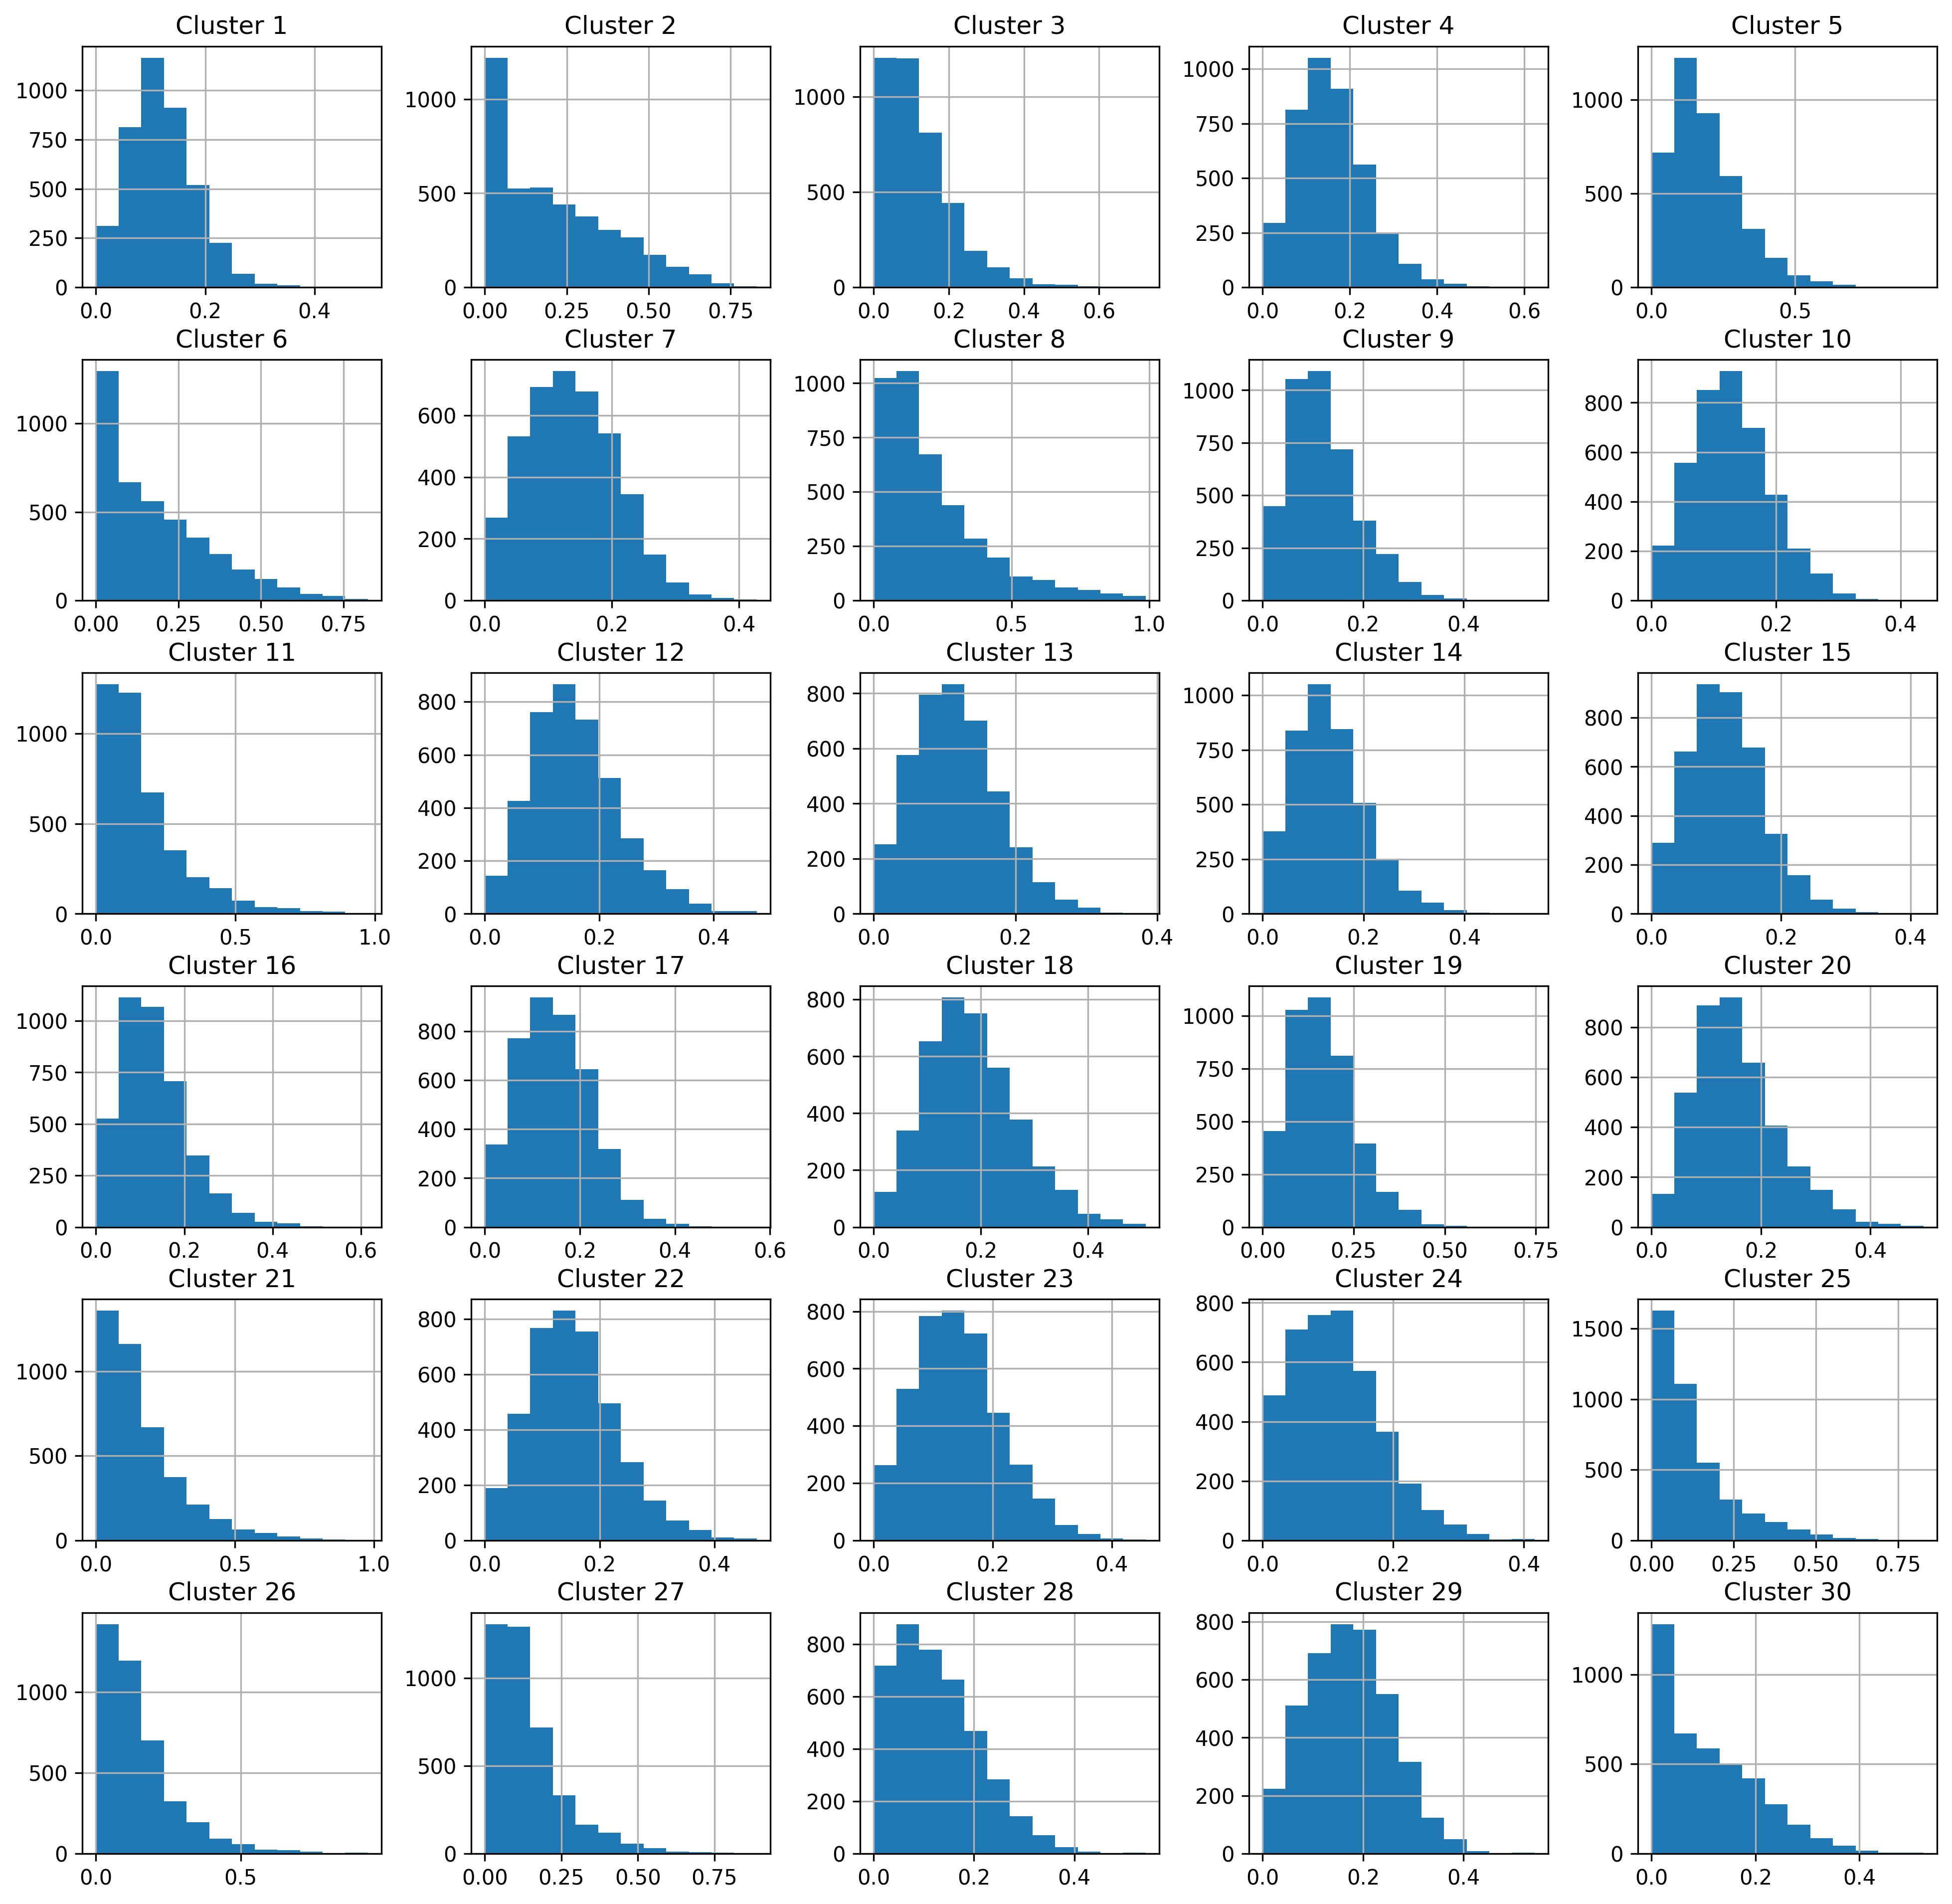
\includegraphics[width=\textwidth]{images/1/1-data_analysis-feature_representation.png}}
        \captionsetup{width=0.9\linewidth}
        \captionsetup{justification=centering}
        \caption{Histogram for each cluster.}
    \end{subfigure}
    \hspace{1cm}
    \begin{subfigure}{.45\textwidth}
        \centering
        \fbox{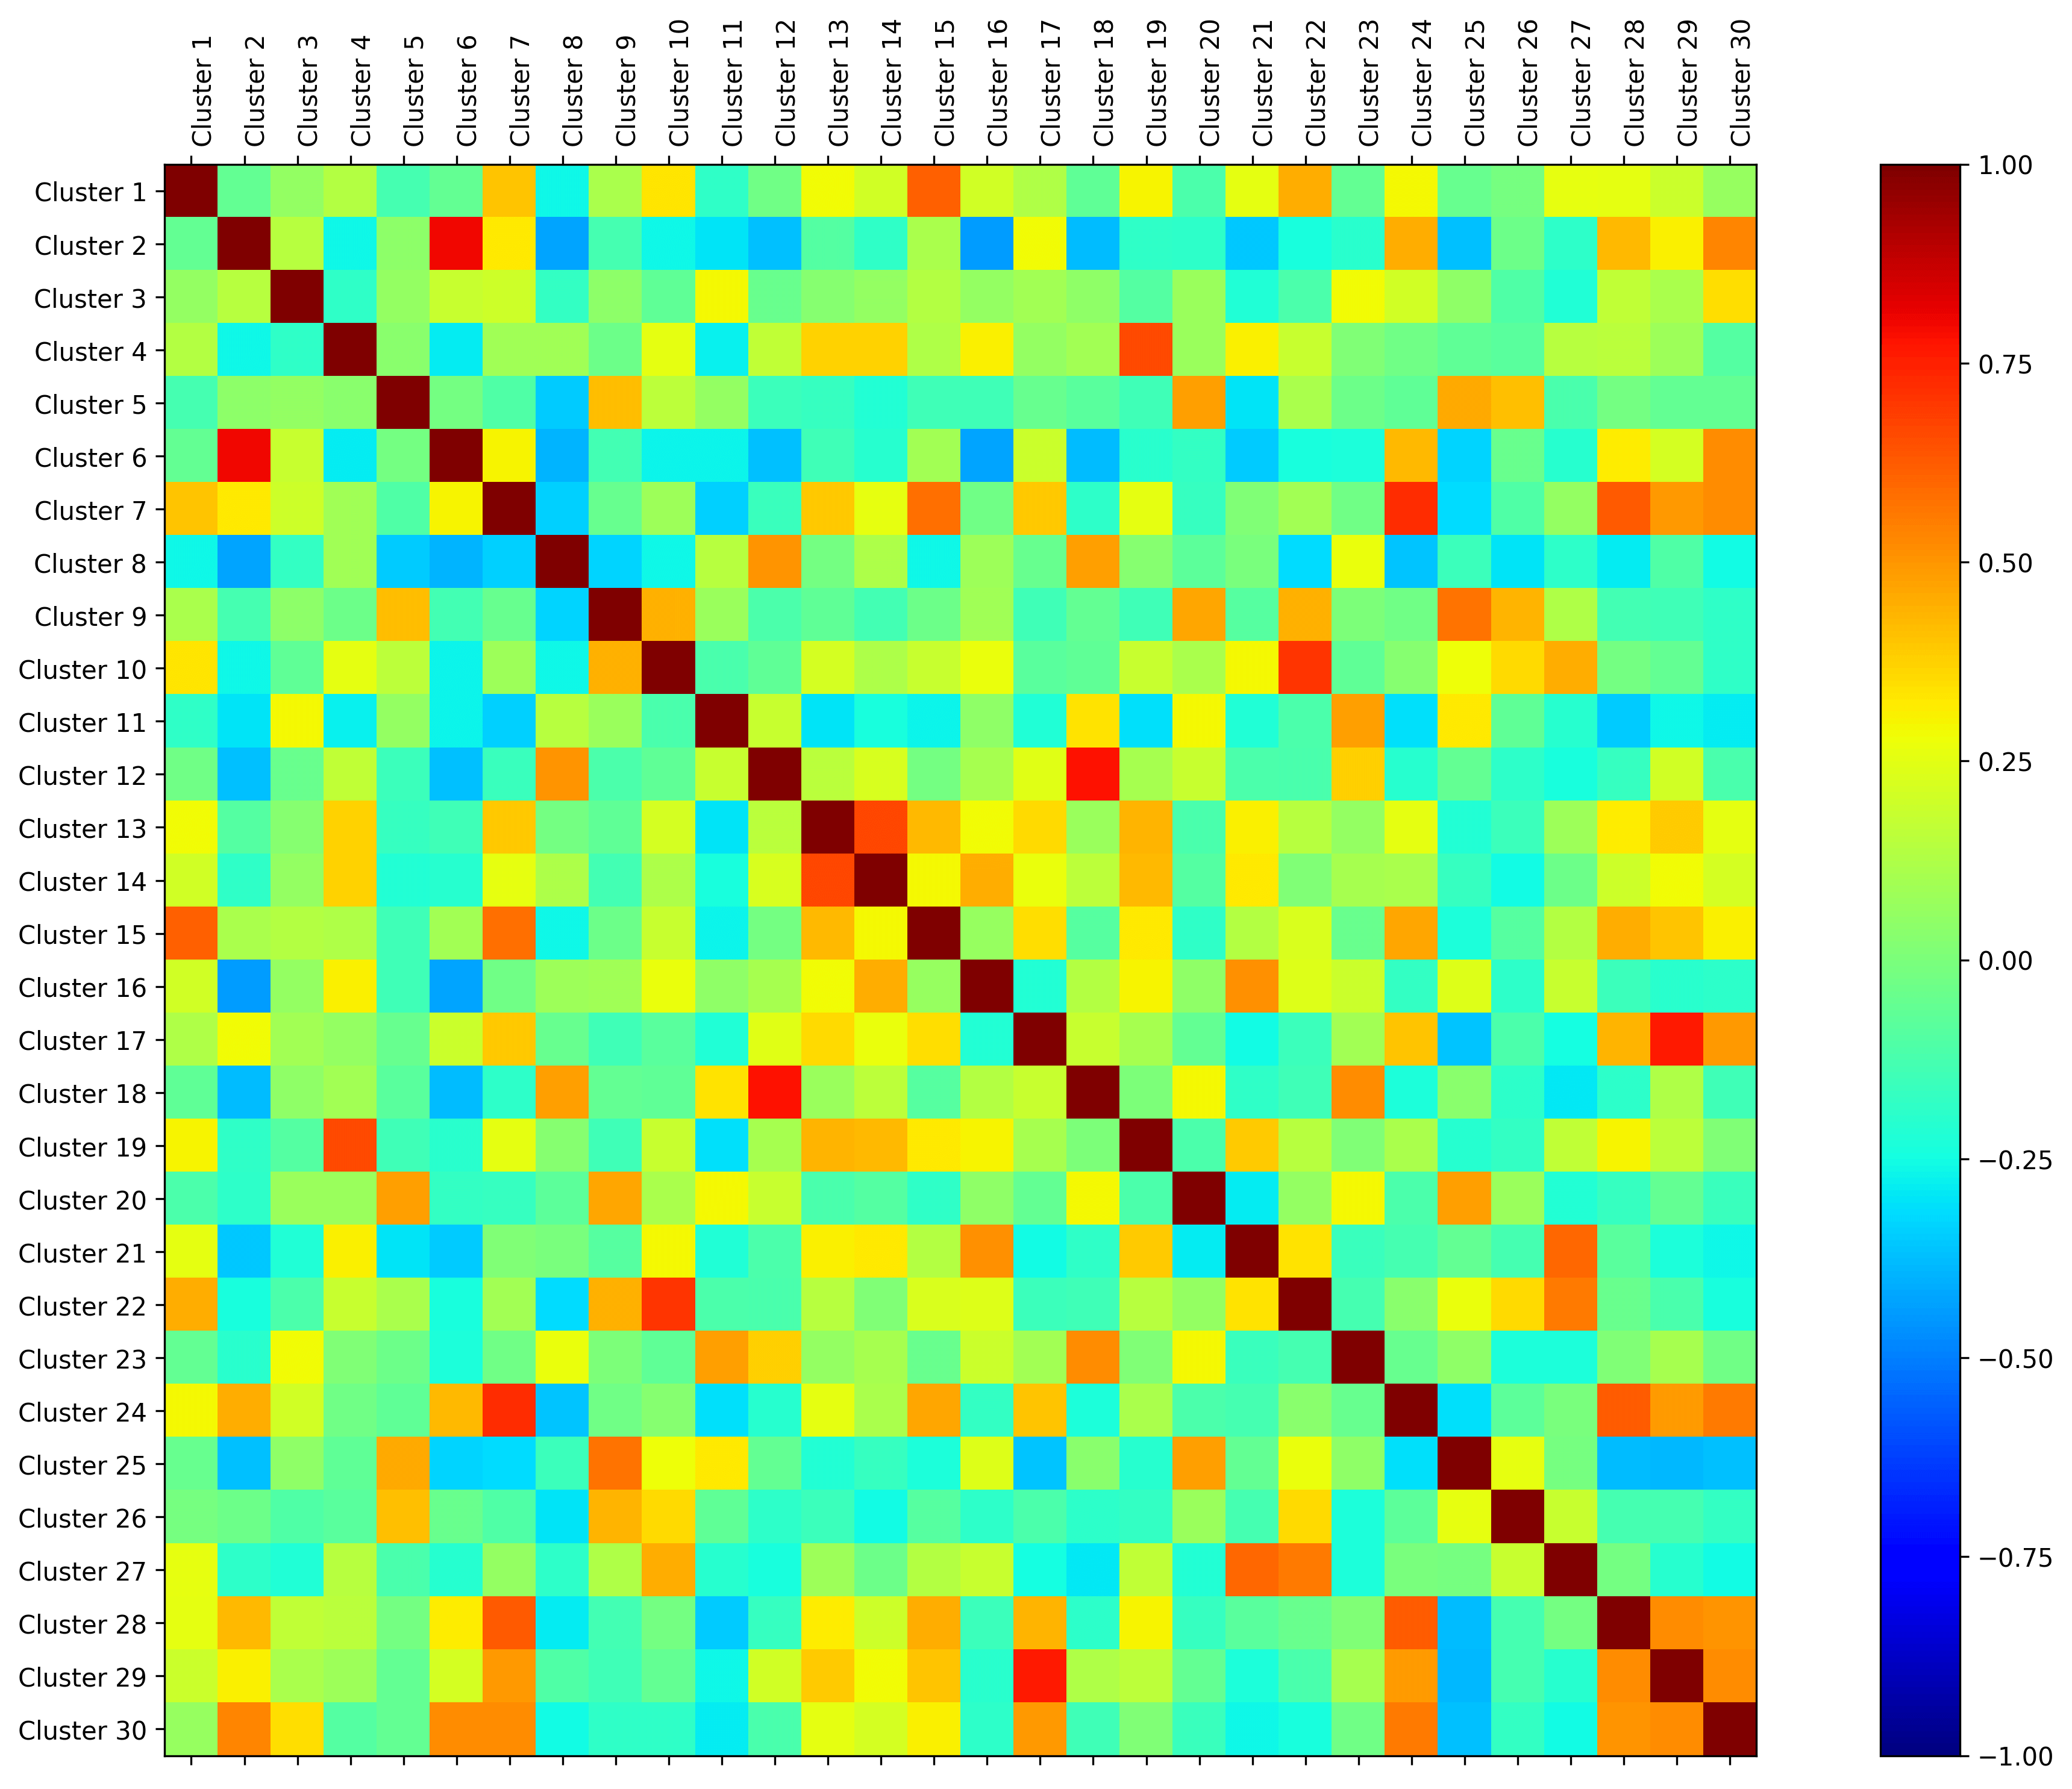
\includegraphics[width=\textwidth]{images/1/1-data_analysis-correlation_matrix.png}}
        \captionsetup{width=0.9\linewidth}
        \captionsetup{justification=centering}
        \caption{Correlation matrix for all clusters.}
    \end{subfigure}
    \captionsetup{width=0.8\linewidth}
    \captionsetup{justification=centering}
    \caption{Data analysis of encoded images using 30 clusters.}
    \label{fig:1-cm}
\end{figure*}